\documentclass[a4paper,11pt]{article}
\usepackage[a4paper,margin=1in]{geometry}
\usepackage{amsmath,amssymb}
\usepackage{booktabs}
\usepackage{graphicx}
\usepackage{caption}
\usepackage[hidelinks]{hyperref}

\title{Recall-prediction benchmark: results}
\author{}
\date{\today}

\begin{document}
\maketitle

\section{Setup}
\begin{itemize}
\item \textbf{Datasets.} Anki: 100 users drawn at random from anki-revlogs-10k. Duolingo: all 115,222 users. Anki robustness: two more 100-user samples (seeds 1 and 2).
\item \textbf{Split.} For each user, a cutoff at the 80th percentile of its review days. Reviews before it are TRAIN and later reviews are TEST. Each TEST event is predicted one step ahead from earlier reviews of its card, and parameters are frozen on TRAIN.
\item \textbf{Scored events.} A TEST event that is not a card's first review and whose gap is at least one day. Same-day reviews enter histories but are not scored. Anki: 95,400 events. Duolingo: 1,189,355 events.
\item \textbf{Metrics.} Log loss (main), Brier score, AUC, and expected calibration error (ECE) over ten equal-width bins.
\item \textbf{Uncertainty.} User-clustered paired bootstrap with 1,000 resamples of users: 95\% intervals for Anki and Duolingo, 99\% intervals for the srs-benchmark comparison.
\item \textbf{Models.}
  \begin{itemize}
  \item FSRS-6 (def.): py-fsrs with default weights for every user.
  \item FSRS-6 (opt.): py-fsrs with weights fitted per user on TRAIN reviews.
  \item HLR: half-life regression.
  \item LagLogit (Duolingo only): lagged-outcome logistic baseline.
  \item v1 (MCMC): Bayesian latent-state retention model, sampled by MCMC (GPU port on Duolingo).
  \item v2 and v3 (MAP): hierarchical FSRS-style models fitted by MAP; v3 adds a user-scale penalty, a lagged-outcome term and a card effect.
  \item GBDT: LightGBM on review-level history features.
  \end{itemize}
\item \textbf{Constant floors.} Three floors fitted on TRAIN rows only, with smoothing pseudo-count $m = 10$: constant (global), constant (per user), and constant (per user, smoothed).
\end{itemize}

\section{Overall results}
On Anki and on Duolingo, GBDT has the best value on every metric among the non-constant models.
Table~\ref{tab:overall} gives the full comparison.

% Generated by paper/scripts/make_tables.py from paper/data/*_overall.csv. Do not edit.
\begin{table*}[t]
\centering
\caption{Overall metrics on Anki and Duolingo. Constants (top three rows) are floors: Const. global, Const. user, and Const. user (sm.), the per-user constant shrunk towards the global rate. FSRS-6 def. and opt. are FSRS-6 with default and optimised weights. v1 (MCMC) is the same Bayesian model on both datasets: the CPU MCMC on Anki and its GPU port on Duolingo. v2 and v3 are MAP fits. Bold: best non-constant model per column. Log loss (LL), Brier and ECE: lower is better; AUC: higher is better.}
\label{tab:overall}
\small
\setlength{\tabcolsep}{4pt}
\begin{tabular}{l rrrr rrrr}
\toprule
 & \multicolumn{4}{c}{Anki} & \multicolumn{4}{c}{Duolingo} \\
\cmidrule(lr){2-5}\cmidrule(lr){6-9}
Model & LL & Brier & AUC & ECE & LL & Brier & AUC & ECE \\
\midrule
Const. global (floor) & 0.454 & 0.141 & 0.500 & 0.004 & 0.279 & 0.074 & 0.500 & 0.003 \\
Const. user (floor) & 0.431 & 0.135 & 0.669 & 0.031 & 0.372 & 0.075 & 0.610 & 0.021 \\
Const. user (sm.) (floor) & 0.431 & 0.135 & 0.669 & 0.031 & 0.272 & 0.072 & 0.615 & 0.008 \\
\midrule
FSRS-6 def. & 0.396 & 0.121 & 0.745 & 0.012 & 0.302 & 0.078 & 0.566 & 0.051 \\
FSRS-6 opt. & 0.379 & 0.117 & 0.777 & 0.009 & 0.300 & 0.078 & 0.570 & 0.051 \\
HLR & 0.680 & 0.170 & 0.555 & 0.146 & 0.418 & 0.079 & 0.521 & 0.072 \\
LagLogit & not run & not run & not run & not run & 0.291 & 0.076 & 0.653 & 0.020 \\
v1 (MCMC) & 0.422 & 0.131 & 0.692 & 0.025 & 0.268 & 0.071 & 0.656 & 0.014 \\
v2 (MAP) & 0.379 & 0.117 & 0.778 & 0.013 & 0.289 & 0.075 & 0.609 & 0.035 \\
v3 (MAP) & 0.378 & 0.117 & 0.779 & 0.010 & 0.283 & 0.074 & 0.613 & 0.032 \\
GBDT & \textbf{0.358} & \textbf{0.111} & \textbf{0.805} & \textbf{0.005} & \textbf{0.259} & \textbf{0.070} & \textbf{0.697} & \textbf{0.001} \\
\bottomrule
\end{tabular}
\end{table*}


\section{Paired differences}
Negative differences favour the model.
A difference is significant only when its interval excludes zero.

% Generated by paper/scripts/make_tables.py from paper/data/*_paired.csv and *_wins.csv. Do not edit.
\begin{table*}[t]
\centering
\caption{Paired log-loss differences (model minus reference; negative favours the model) with 95\% user-clustered bootstrap CIs, and the share of users whose log loss is lower for the model than for FSRS-6 (opt.). Reference: FSRS-6 (opt.) and the smoothed per-user constant.}
\label{tab:paired}
\small
\setlength{\tabcolsep}{4pt}
\resizebox{\textwidth}{!}{%
\begin{tabular}{l ccc ccc}
\toprule
 & \multicolumn{3}{c}{Anki} & \multicolumn{3}{c}{Duolingo} \\
\cmidrule(lr){2-4}\cmidrule(lr){5-7}
Model & vs FSRS-6 opt. & vs const. sm. & user win & vs FSRS-6 opt. & vs const. sm. & user win \\
\midrule
v1 (MCMC) & +0.043 [+0.033, +0.055] & $-$0.009 [$-$0.014, $-$0.004] & 22\% & $-$0.032 [$-$0.033, $-$0.031] & $-$0.004 [$-$0.004, $-$0.004] & 74\% \\
v3 (MAP) & $-$0.001 [$-$0.004, +0.002] & $-$0.053 [$-$0.067, $-$0.041] & 58\% & $-$0.017 [$-$0.018, $-$0.016] & +0.011 [+0.010, +0.011] & 72\% \\
GBDT & $-$0.021 [$-$0.028, $-$0.014] & $-$0.072 [$-$0.089, $-$0.058] & 82\% & $-$0.042 [$-$0.042, $-$0.041] & $-$0.013 [$-$0.014, $-$0.013] & 78\% \\
FSRS-6 opt. & -- & $-$0.051 [$-$0.067, $-$0.039] & -- & -- & +0.028 [+0.027, +0.029] & -- \\
\bottomrule
\end{tabular}}
\end{table*}


\section{Gap bins}
Duolingo's scored gaps reach at most 11 days, so only the 1d, 2--3d and 4--14d bins are populated.

\begin{figure}[t]
\centering
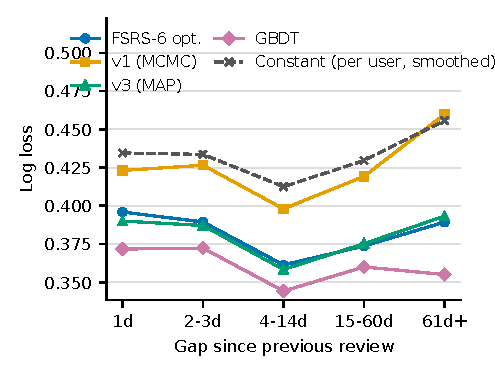
\includegraphics[width=0.85\textwidth]{figures/gaps_anki}
\caption{Log loss by gap bin on Anki, for FSRS-6 (opt.), v1 (MCMC), v3 (MAP), GBDT and the constant (per user, smoothed). Lower is better. Bins are 1d, 2-3d, 4-14d, 15-60d and 61d+ gaps; a bin is drawn only if it holds scored events.}
\label{fig:gaps-anki}
\end{figure}

\begin{figure}[t]
\centering
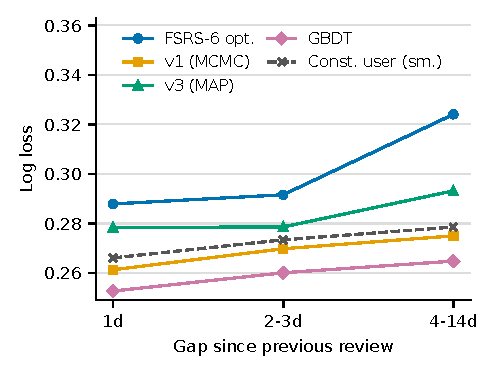
\includegraphics[width=0.85\textwidth]{figures/gaps_duolingo}
\caption{Log loss by gap bin on Duolingo, for the same five series. Lower is better. Only the 1d, 2-3d and 4-14d bins hold scored events, so only those are drawn.}
\label{fig:gaps-duolingo}
\end{figure}

\section{Calibration}
Each point in the reliability diagrams is one of ten equal-width bins of predicted recall, plotted at the mean prediction (x) and the observed recall (y).
Among the non-constant models on Anki, GBDT has the lowest ECE (0.0049).

\begin{figure}[t]
\centering
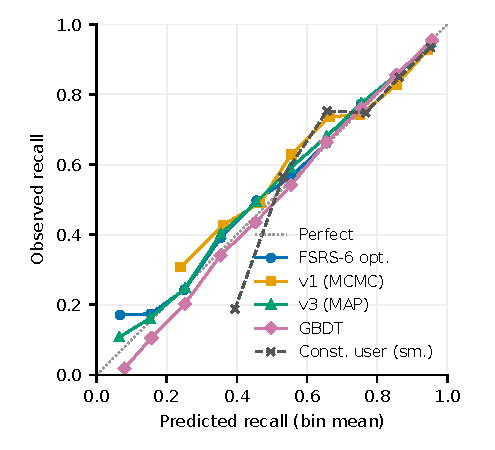
\includegraphics[width=0.85\textwidth]{figures/reliability_anki}
\caption{Reliability diagram on Anki for FSRS-6 (opt.), v1 (MCMC), v3 (MAP), GBDT and the constant (per user, smoothed). Each point is one of ten equal-width bins of predicted recall, plotted at the mean prediction (x) and the observed recall (y). The dotted line is perfect calibration. Bins with fewer than 30 reviews are omitted.}
\label{fig:rel-anki}
\end{figure}

\begin{figure}[t]
\centering
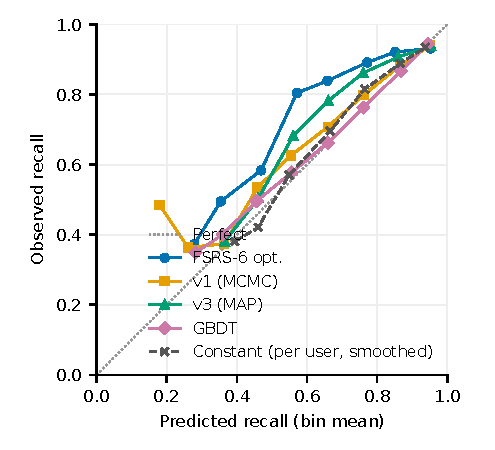
\includegraphics[width=0.85\textwidth]{figures/reliability_duolingo}
\caption{Reliability diagram on Duolingo for the same five series, with the same binning. The dotted line is perfect calibration. Bins with fewer than 30 reviews are omitted.}
\label{fig:rel-duolingo}
\end{figure}

\section{Robustness across Anki samples}
GBDT is better than FSRS-6 (opt.) on each of the three 100-user samples.
Per-seed log-loss differences are $-$0.0210, $-$0.0226 and $-$0.0210, and each interval excludes zero.

% The seeds table has long interval cells; it is set one size smaller to fit the text width.
\begingroup\renewcommand{\small}{\footnotesize}% Generated by paper/scripts/make_tables.py from paper/data/anki_seeds*.csv. Do not edit.
\begin{table*}[t]
\centering
\caption{Anki robustness: log loss on three 100-user samples (seeds 0, 1, 2). The GBDT row gives the per-seed difference GBDT minus FSRS-6 (opt.) with its 95\% CI. v1 and v2 are not part of the robustness runs.}
\label{tab:seeds}
\small
\setlength{\tabcolsep}{3pt}
\begin{tabular}{l rrr r}
\toprule
Model & Seed 0 & Seed 1 & Seed 2 & Mean \\
\midrule
Const. global & 0.454 & 0.393 & 0.433 & 0.427 \\
Const. user & 0.431 & 0.361 & 0.406 & 0.399 \\
FSRS-6 def. & 0.396 & 0.325 & 0.364 & 0.362 \\
FSRS-6 opt. & 0.379 & 0.314 & 0.352 & 0.349 \\
HLR & 0.680 & 0.555 & 0.595 & 0.610 \\
v3 (MAP) & 0.378 & 0.308 & 0.351 & 0.346 \\
GBDT & 0.358 & 0.292 & 0.331 & 0.327 \\
\midrule
GBDT $-$ FSRS-6 opt. & $-$0.021 [$-$0.028, $-$0.014] & $-$0.023 [$-$0.037, $-$0.014] & $-$0.021 [$-$0.033, $-$0.012] & $-$0.022 \\
\bottomrule
\end{tabular}
\end{table*}
\endgroup

\section{srs-benchmark comparison}
The pooled GBDT is trained on 450 users, with 50 more for early stopping, all disjoint from the 1,000 evaluation users (ids 1--1,000).
Boosting reached the 2,000-round cap, so its numbers are a lower bound.

% Generated by paper/scripts/make_tables.py from paper/data/srsb*.csv. Do not edit.
\begin{table*}[t]
\centering
\caption{srs-benchmark comparison on 1,000 evaluation users (ids 1--1,000), with the benchmark's own split and metrics. Published results are from the benchmark repository. GBDT is pooled: it is trained on other users, not per user. Unweighted values are per-user means, as in the benchmark README; weighted values weight each user by its number of test rows. The last column is the size-weighted log-loss difference GBDT minus the model (negative favours GBDT) with a 99\% user-clustered bootstrap CI. A dash means that no paired interval is in the export.}
\label{tab:srsb}
\small
\setlength{\tabcolsep}{4pt}
\begin{tabular}{l rrr r}
\toprule
 & \multicolumn{2}{c}{LogLoss} & AUC & GBDT $-$ model \\
\cmidrule(lr){2-3}
Model & unweighted & weighted & unweighted & size-weighted [99\% CI] \\
\midrule
GBDT (ours, pooled) & 0.3211 & 0.3148 & 0.7780 & -- \\
RWKV-Instant & 0.2860 & 0.2828 & 0.8319 & +0.0320 [+0.0287, +0.0358] \\
RWKV-Curve & 0.3302 & 0.3143 & 0.7665 & +0.0006 [$-$0.0044, +0.0055] \\
GRU & 0.3441 & 0.3271 & 0.7298 & $-$0.0123 [$-$0.0174, $-$0.0067] \\
LSTM & 0.3445 & 0.3271 & 0.7311 & -- \\
MOVING-AVG & 0.3462 & 0.3372 & 0.7007 & $-$0.0224 [$-$0.0255, $-$0.0196] \\
FSRS-7 recency & 0.3485 & 0.3308 & 0.7208 & -- \\
Logistic Regression & 0.3502 & 0.3341 & 0.7090 & -- \\
FSRS-6 & 0.3580 & 0.3383 & 0.6994 & $-$0.0235 [$-$0.0286, $-$0.0183] \\
AVG & 0.4055 & 0.3802 & 0.5007 & $-$0.0654 [$-$0.0730, $-$0.0587] \\
HLR & 0.4877 & 0.4479 & 0.6352 & -- \\
\bottomrule
\end{tabular}
\end{table*}


\section{Caveats}
\begin{itemize}
\item \textbf{v1 (MCMC) did not converge.} Its decay parameter has split R-hat 2.44 on Anki and 2.48 on Duolingo, with effective sample sizes 3.05 and 3.00. Its results are provisional.
\item \textbf{FSRS-6 (opt.) mostly uses default weights on Duolingo.} It falls back to default weights for 115,110 of 115,222 users.
\item \textbf{The test set was looked at twice.} v2 was tested in one round. v3 and GBDT were tested together in a second round, after GBDT was frozen on validation.
\item \textbf{RWKV-Instant uses extra features.} This makes it not a like-for-like comparison.
\end{itemize}

\end{document}
